\section{Detailed Implementation}
\label{section:implementation}
Please explain your implementation in detail. You may do this with the help of pseudo code or a figure of system architecture. Please also highlight which parts of the algorithm lead to the most difficulty in your implementation.


\textbf{taxi domain:}

\begin{figure}[htbp]
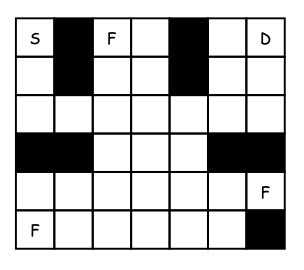
\includegraphics[width=0.25\textwidth]{taxi.png}
\end{figure}

environment:
In this experience, s is the starting position, d is the destination, and f represents passenger, it will get +1 reward for delivering one passenger, +3 for two , +15 for three.
\\
\\
we preform SARSA with epsilon-greedy, SARSA with Boltzmann softmax and SARSA with Mellowmax softmax. In this environment, there are 33 posible positions and three passengers, therefore, it has 33*2*2*2 = 264 states and four possible actions.
\\
\\
In our algorithm, we set some prohibited state-action pair's Q values to negative infinity, like hit the wall. Moreover, durning the training period, we will not choose those action in order not to affect other Q values.
\\
\\
Because this environment need to have proper exploration, therefore, Boltzmann and Mellowmax can show their advantage. However, there are some detail that not be mention in this paper, so we have our own setting.
\\
\\
In epsilon-greedy method, training and testing both use epsilon-greedy to select action. And in Boltzmann softmax, training and test both use Blotzmann too. However, in Mellowmax softmax, we use Mellowmax softmax durning training process, and in testing process, we select the actions which have max Q values according to our pre-train Q values. We found that there are more approximate to paper's results.